% Copyright © 2022 LMU Munich Media Informatics Group. All rights reserved.
% Created by Changkun Ou <https://changkun.de>.
%
% Use of this source code is governed by a GNU GPLv3 license that
% can be found in the LICENSE file.

% This tex file generates a combined PDF file for Figure 5.
%
% Usage:
%
% latexmk -pdf dist.tex --jobname=fig5 && mv fig5.pdf ../assets/fig5_all.pdf && latexmk -c

\documentclass{standalone}
\usepackage{color}
\usepackage{graphicx}
\usepackage{tikz}

\begin{document}
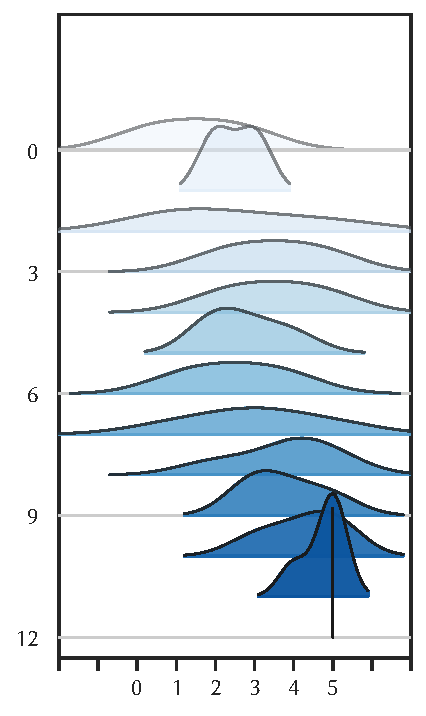
\includegraphics[width=0.23\textwidth]{../assets/ratingdist/ideal2.pdf}
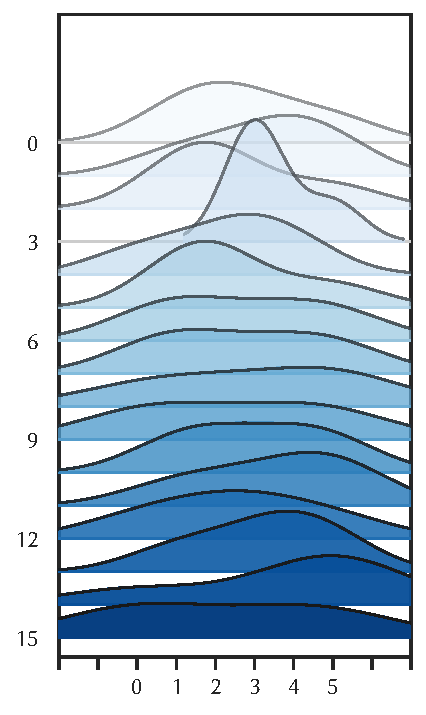
\includegraphics[width=0.23\textwidth]{../assets/ratingdist/dacdd183-4dd0-11ec-86eb-a85e4557a9b6.pdf}
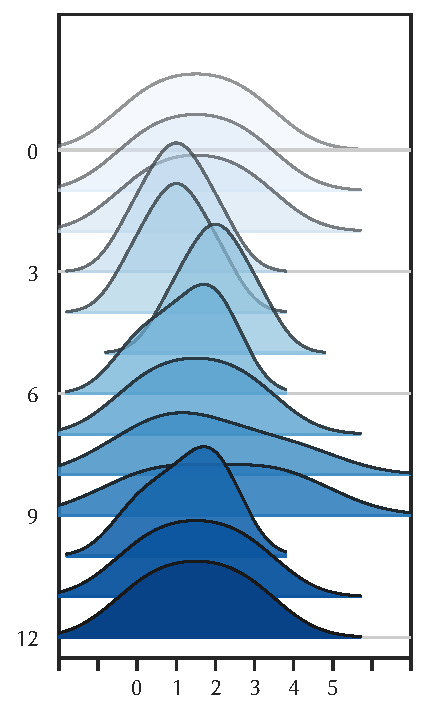
\includegraphics[width=0.23\textwidth]{../assets/ratingdist/48f9c537-43f4-4a22-a7ff-4ce8d9e48d4e.pdf}
\begin{tikzpicture}
    \pgftext{
    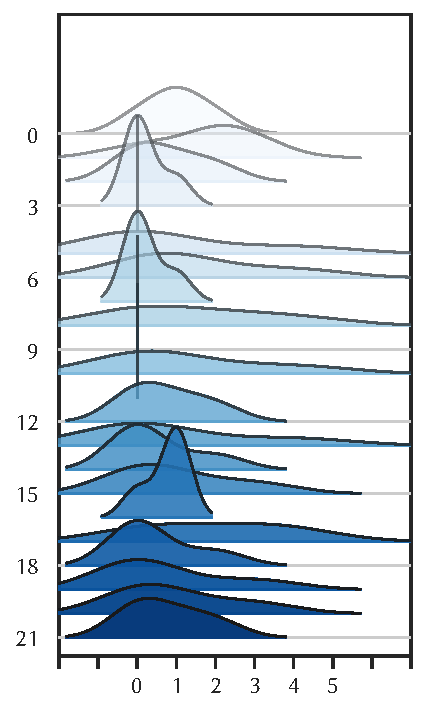
\includegraphics[width=0.23\textwidth]{../assets/ratingdist/086d8b7a-fa86-4b80-93b7-1a40fed9bc80.pdf}
    }
    \draw[<-] (2.18,-2) -- (2.18,2);
    \node[rotate=-90] at (2.3,0) {\scriptsize time (iteration)};
\end{tikzpicture}
\end{document}